%
% File: chap01.tex
% Author: Victor F. Brena-Medina
% Description: Introduction chapter where the biology goes.
%
\let\textcircled=\pgftextcircled
\chapter{Self-Priming Dielectric Elastomer Generators}
\label{chap:2}

\initial{T}his chapter is partially based on the proceeding published 

One of the main challenges for the practical implementation of dielectric elastomer generators (DEGs) is supplying high voltages. To address this issue, systems using self-priming circuits (SPCs) --- which exploit the DEG voltage swing to increase its supplied voltage --- have been used with success. 
A self-priming circuit consists of a charge pump implemented in parallel with the DEG circuit. At each energy harvesting cycle, the DEG receives a low voltage input and, through an almost constant charge cycle, generates a high voltage output. SPCs receive the high voltage output at the end of the energy harvesting cycle and supply it back as input for the following cycle, using the DEG as a voltage-multiplier element.
 Although rules for designing self-priming circuits for dielectric elastomer generators exist, they have been obtained from intuitive observation of simulation results and lack a solid theoretical foundation.
Here we report the development of a mathematical model to predict voltage boost using self-priming circuits. The voltage on the DEG attached to the SPC is described as a function of its initial conditions, circuit parameters/layout, and the DEG capacitance. Our mathematical model has been validated on an existing DEG implementation from the literature, and successfully predicts the voltage boost for each cycle. Furthermore, it allows us to understand the conditions for the boost to exist, and obtain the design rules that maximize the voltage boost.

%=======
\section{Introduction}
\label{sect:intro}  % \label{} allows reference to this section
\paragraph{} According to the World Energy Council\cite{EnergyIssues}, 1.2 billion people do not have access to electricity. Energy price volatility and greenhouse gas emissions issue accentuate this issue, and point to the need for cheap, reliable and renewable energies.  As a new and emerging eletromechanical energy conversion technology, Dielectric Elastomer Generators (DEGs) are one possible solution. With low frequency and wide bandwidth\cite{Boots2buoys}, energy harvesting DEGs have already been reported for use in wave energy generation \cite{VertechyPolyWECtest2014}, human motion energy harvesting\cite{MistralHMotion2008} and even as thermal machines\cite{Boots2buoys}.
\paragraph{} DEGs harvest energy through capacitance change induced by  deformation. The energy harvesting happens in cycles; one example with four stages I--IV is illustrated in Figure \ref{fig:cycle}. The transitions between states in this cycle are as follows.
\begin{itemize}
\item I$\rightarrow$II: From an initially relaxed phase, the DEG is stretched by a mechanical load and increases its capacitance.
\item II$\rightarrow$III: Once stretched, the DEG is polarized through an electrical energy input.
\item III$\rightarrow$IV: From stretched and polarized, in an open circuit configuration, the mechanical load is released letting the material relax, so reducing the DEG's capacitance. As the capacitance reduces and the charge stored is maintained constant, there is a voltage rise.
\item IV$\rightarrow$I: Finally, the DEG is discharged from its more energetic state, back to its initial state.
\end{itemize}

\begin{figure}[ht]
\begin{center}
\begin{tabular}{c}
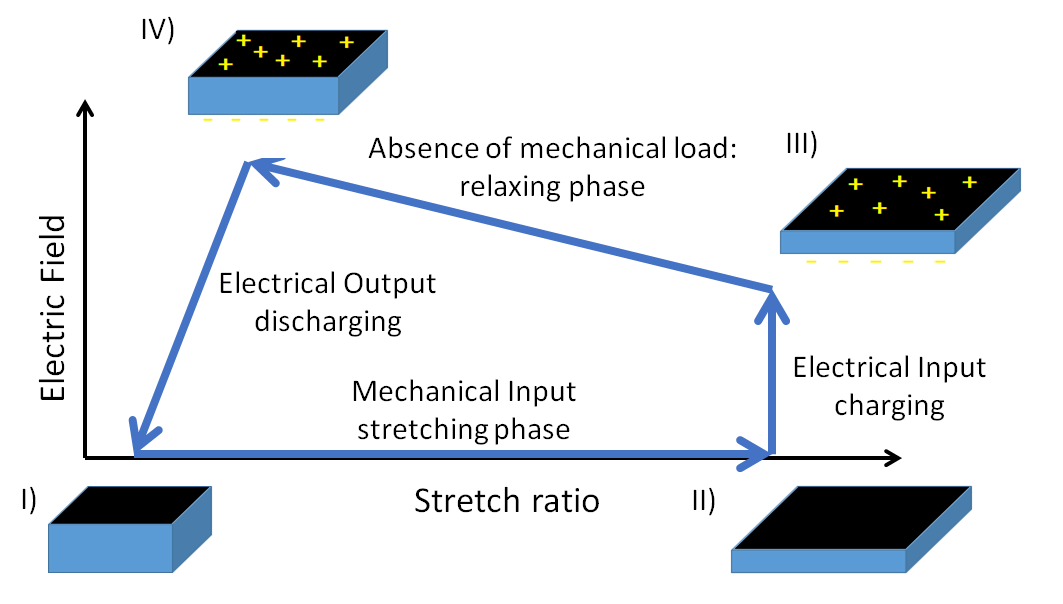
\includegraphics[height=6cm]{Cycle.png}
\end{tabular}
\end{center}
\caption 
{ \label{fig:cycle}
DEG energy harvesting cycle using relaxation with constant charge} 
\end{figure} 

\paragraph{} Among the drawbacks of current DEG technology is the necessary condition of inputting electrical energy to polarize the material. Furthermore, the energy output between states IV and I is proportional to the amount of electrical energy used to polarize the DEG between states II and III\cite{DEGCycles}, so, in order to explore the energy harvesting capabilities at its maximum, one might want to input high voltages.

\paragraph{} A solution for generating the high voltage in DEGs is the use of Self-priming Circuits (SPCs), proposed by McKay \textit{et al.}\cite{SPC2010}. An SPC consists of an inverse charge pump, toggling between high and low capacitance states, depending on its polarization. The circuit is composed of diodes and capacitors, as illustrated in Figure \ref{fig:spc}.  An SPC can be polarized in a High Voltage (HV) form, which has a lower capacitance and will only allow current to charge the capacitors, or in a High Charge (HC) state, which has higher capacitance and will only allow current to flow from the SPC (considering their poles are connected such that $V_A > V_B$).

\begin{figure}[ht]
\begin{center}
\begin{tabular}{c}
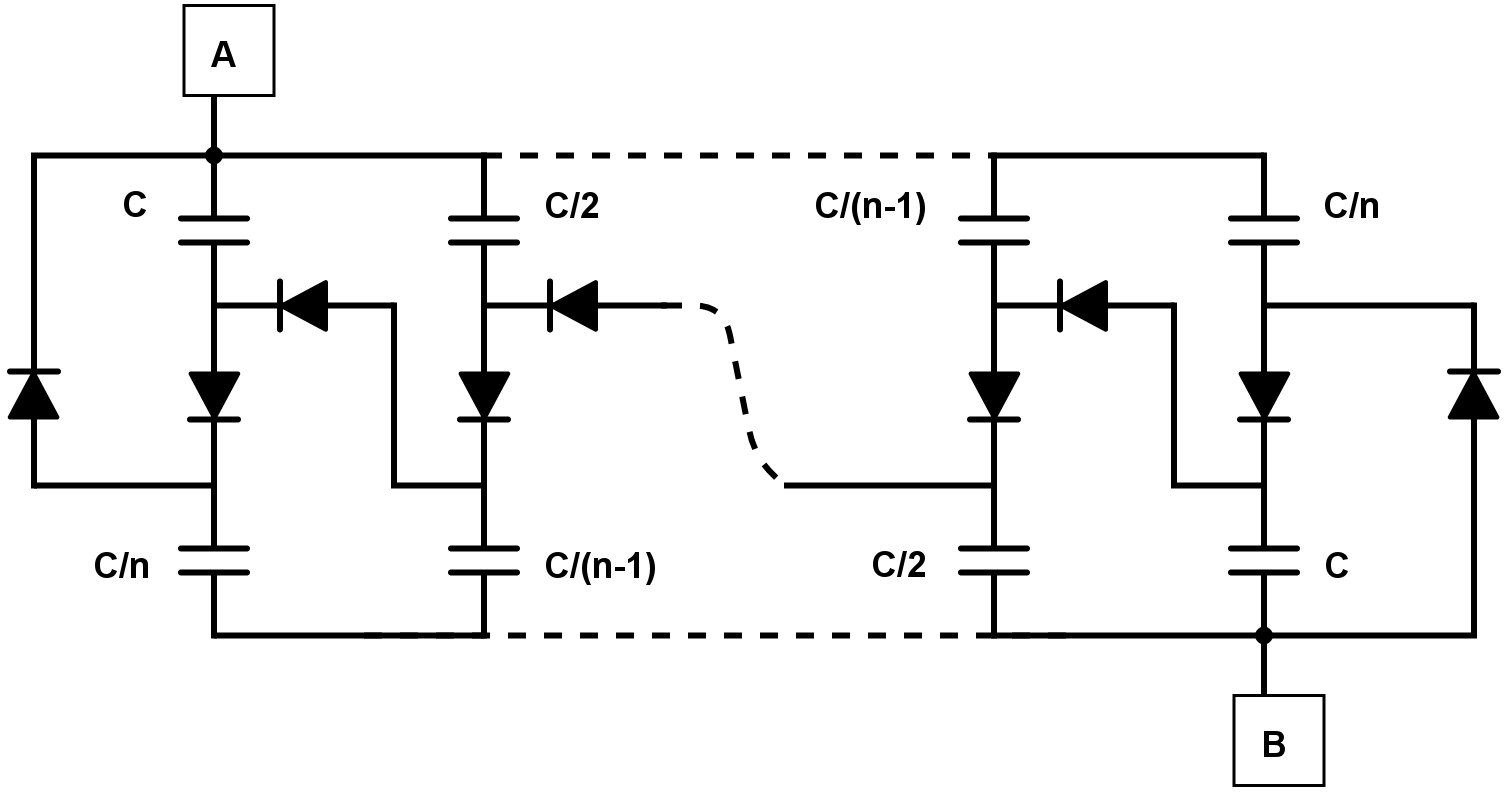
\includegraphics[height=5.2cm]{SPC_general.png}
\end{tabular}
\end{center}
\caption 
{ \label{fig:spc}
SPC general scheme. Adapted from McKay \textit{et al.}\cite{SPCdesign}. } 
\end{figure} 

\begin{figure}[ht]
\begin{center}
\begin{tabular}{c}
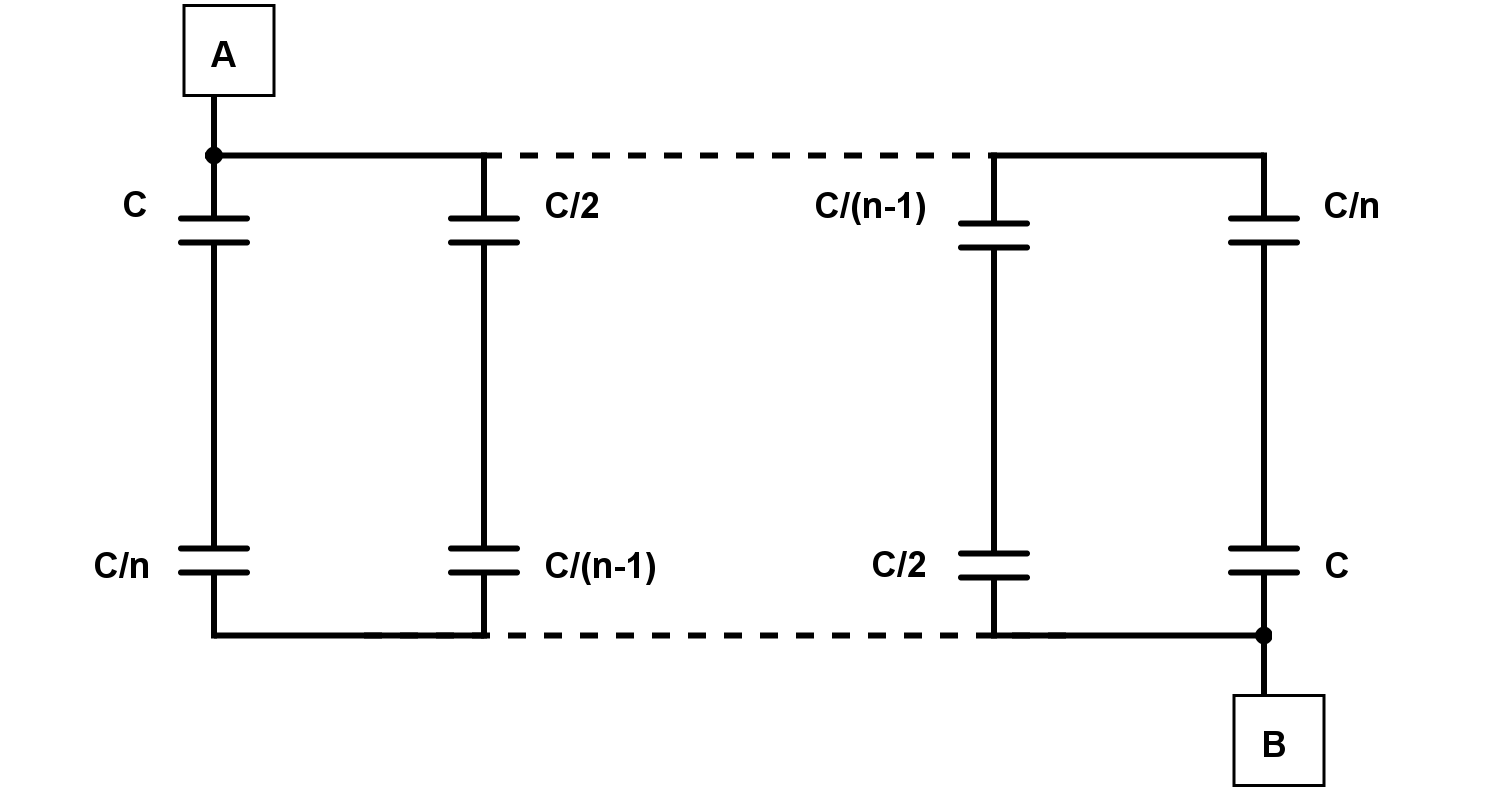
\includegraphics[height=4.2cm]{SPC_HV3.png}
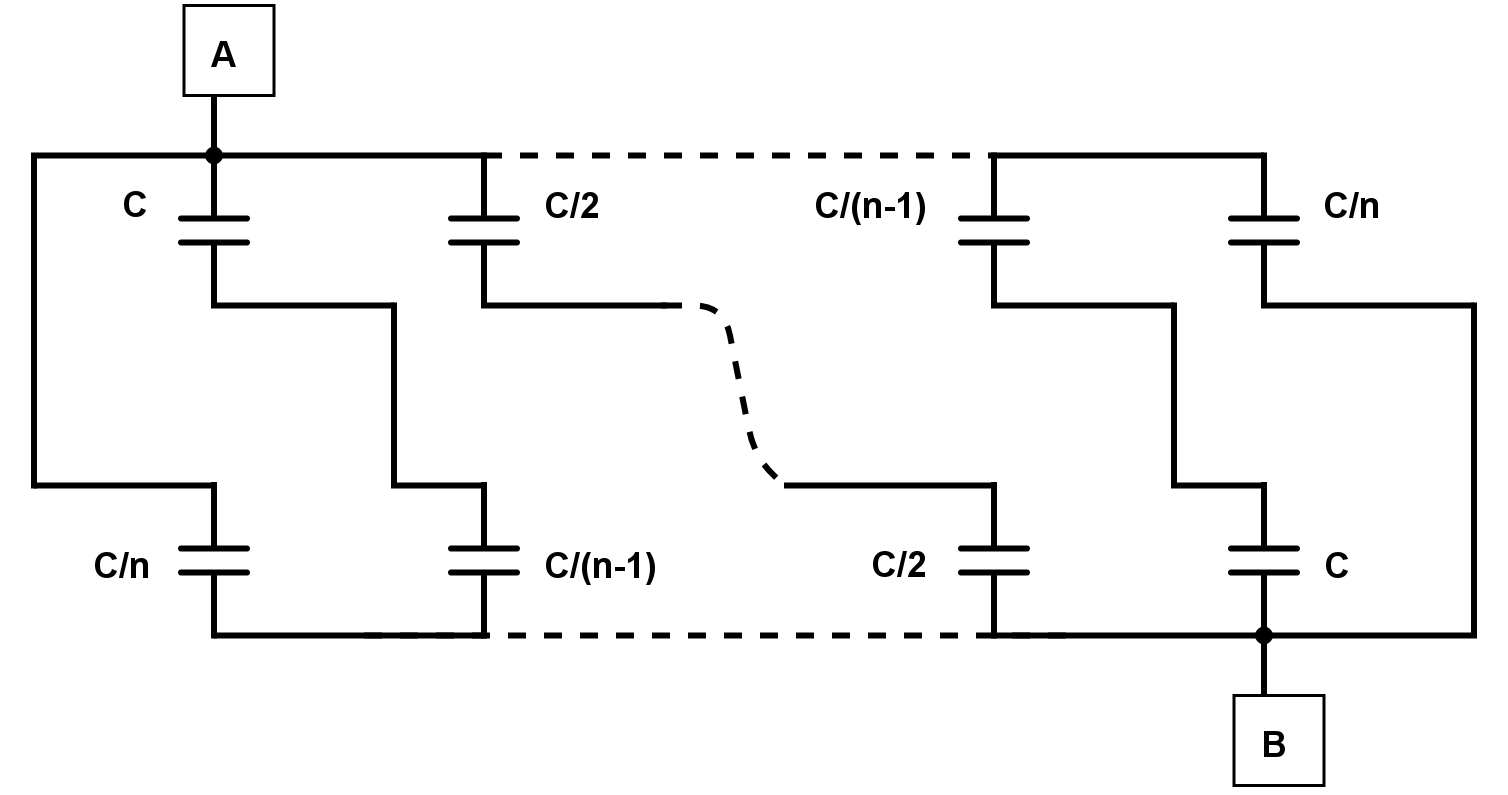
\includegraphics[height=4.2cm]{SPC_HC3.png}\\
(a) \hspace{7cm} (b)
\end{tabular}
\end{center}
\caption 
{ \label{fig:spc_form}
SPC effective configuration with (a) HV polarization, and (b) HC polarization. Adapted from McKay \textit{et al.}\cite{SPCdesign}.} 
\end{figure} 

\paragraph{} The advantage of using an SPC is that it allows part of the energy output in a DEG cycle to be stored and used as an input in the following one. Through the use of an SPC it is possible to initially prime the DEG-SPC system with low voltage and, by cycles of stretching-relaxing the DEG, bring the system to high voltage and increase its energy output.

\paragraph{}SPCs have been a promising topic of research, and upgrades have been made to their layout (see Figure \ref{fig:spc}), such as using antagonistic DEG membranes to replace the capacitors normally used\cite{AntagSPC}, or the use of Dielectric Elastomer Switches (DES), which are flexible resistive  elements incorporated in the membrane that are able to toggle between high and low resistance, and replace the diodes in the SPC\cite{DESSPC}.

\paragraph{}Here, we report a mathematical model of the simple SPC-DEG system and, through it, provide general design rules. Although design rules have already been suggested \cite{SPCdesign}, they appear to have been based on intuitive observation of numerical simulation results. We will derive analytic expressions for the rules, and demonstrate why they work and how they can be improved, with the overall aim of better understanding the SPC as a voltage-boosting element that can solve the high-energy input issue in DEG cycles.

\section{Self-priming circuits}

\paragraph{}  As described previously for the DEG energy harvesting cycle, the DEG-SPC system also passes through different phases during the DEG stretch-relax cycle. These cycle phases and the model assumptions are detailed below; the resulting voltage and capacitance are shown in Figure \ref{fig:cycleph}.

\subsection{Cycle phases}

\paragraph{} Using an SPC connected in parallel with the  DEG, we can increase the voltage every time the DEG is cycled.  Note that the voltages represented in Figure \ref{fig:cycleph} for the HV and HC forms reflect the voltage if the SPC was simply a capacitor with constant capacitance with a certain amount of charge stored. However, given the arrangement of the diodes,  charge only flows into the SPC in its HV form and from it in its HC form.  If we consider a DEG stretch-relax cycle between fixed  maximum and minimum stretch, we can describe the DEG-SPC cycle in four phases (see Figure \ref{fig:SPCcycle}).

\paragraph{Phase 1} Starting from a point similar to stage III described in Figure \ref{fig:cycle}, the DEG capacitance starts decreasing as it relaxes. Given that its voltage is not yet higher than that on the SPC in HV form, charge will not flow to the SPC. Similarly, the DEG voltage is higher than the SPC voltage in its HC form, thus, there is no charge flow from the SPC into the DEG. Consequently, we have a voltage increase in the DEG (similar to the process III$\rightarrow$IV).
\paragraph{Phase 2} As the voltage on the DEG achieves the same level of that in the SPC in its HV form, the DEG starts discharging into the SPC. The DEG voltage keeps rising due to the capacitance decrease, and the SPC voltage rises due to its charging.
\paragraph{Phase 3} Once the DEG stops relaxing and starts being stretched again, its capacitance starts to rise. As a consequence, the voltage starts dropping in the DEG. In an similar situation to Phase 1, there is no charge flow between the SPC and the DEG, as the first has a higher voltage in its HV form and a lower voltage in its HC form, preventing the flow of charge to or from the SPC.
\paragraph{Phase 4} When the voltage in the DEG reaches that of the SPC in its HC form, a charging current starts to flow from the SPC. As the DEG has a capacitance decrease, its voltage keeps dropping. The SPC also loses charge due to drain into the DEG. At the moment the DEG's capacitance stops rising and starts decreasing again, the cycle restarts, going back to Phase 1.


\begin{figure}[ht]
\begin{center}
\begin{tabular}{c}
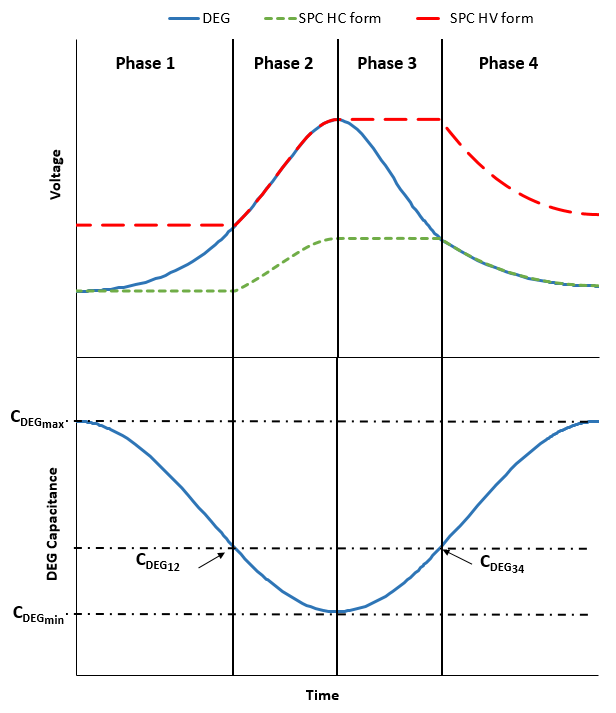
\includegraphics[height=12cm]{Phasestgt2.png}
\end{tabular}
\end{center}
\caption 
{ \label{fig:cycleph}
The four phases of the cycle.} 
\end{figure}

\begin{figure}[ht]
\begin{center}
\begin{tabular}{c}
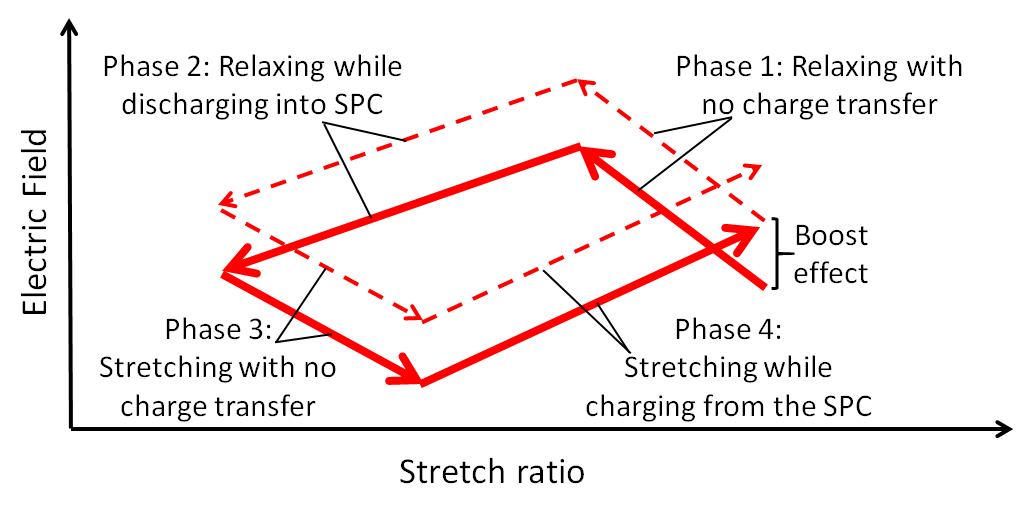
\includegraphics[height=5cm]{SPC_cycle_ph2.png}\\
\end{tabular}
\end{center}
\caption 
{ \label{fig:SPCcycle}
The DEG-SPC cycle, shown as electric field as a function of stretch.} 
\end{figure}

We can see how the cycle produces an overall system voltage boost in Figure \ref{fig:cycles}, which illustrates the boosting process, showing the DEG-SPC voltage and the voltage in the SPC given by its stored charge and the capacitance on each of its forms. 

\begin{figure}[ht]
\begin{center}
\begin{tabular}{c}
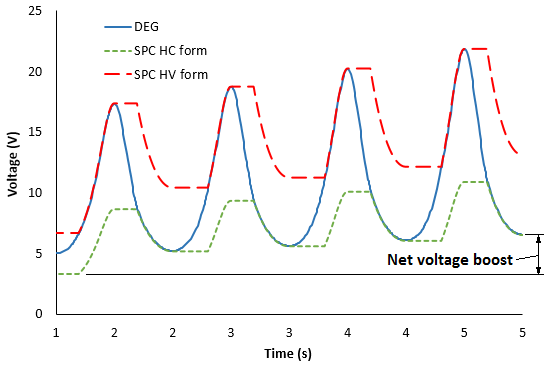
\includegraphics[height=5cm]{Cycles2.png}\\
\end{tabular}
\end{center}
\caption 
{ \label{fig:cycles}
Voltage as a function of time for the DEG and the SPC, in both its HC and HV form.} 
\end{figure}


\subsection{SPC model considerations}
\paragraph{} In the HV form of the SPC there are $n$ branches in parallel, each with capacitance $\ofrac{C}{(n+1)}$, and, in the HC form, there are $n+1$ stages with capacitance $\ofrac{C}{n}$. Thus, the equivalent capacitance of the circuit can be written in each form as: \begin{align}
C_{\text{SPC}_\text{HV}}&=C\left(\frac{n}{n+1}\right),\label{eq:cspchv}\\
C_{\text{SPC}_\text{HC}}&=C\left(\frac{n+1}{n}\right).\label{eq:cspchc}
\end{align}

\paragraph{} Considering the initial situation when the circuit is primed with a voltage $V_0$, in an equilibrium condition (no current flow), we can calculate that each capacitor with capacitance $C$ has a voltage drop of
\begin{equation}
V_{C_{0}}=\frac{2V_{0}}{(2n+1)}.
\end{equation}
This implies that the initial voltage in which the HV form will be active is
\begin{equation}
V_{\text{SPC}_\text{HV}} = (n+1)V_{C_{0}}.
\end{equation}
The same reasoning can be applied to the HC form; the voltage at which it will be triggered is
\begin{equation}
V_{\text{SPC}_\text{HC}} = \frac{n}{n+1}V_{\text{SPC}_\text{HV}}.
\end{equation}

\section{Modeling the boost cycle phases}
In this section we introduce a general model of each phase of the DEG-SPC voltage boosting cycle.  Figure \ref{fig:circuit} illustrates the high-level circuit scheme of the DEG-SPC system, attached to a load. The source $V_0$ is used only to supply an initial priming for the DEG-SPC system and the diode prevents charge to flow back through it when the voltage boost occurs. For this model, we consider that the DEG stretches and relaxes sinusoidally between two fixed positions, creating maximum and minimum area configurations, thus corresponding to a simple variable capacitor oscillating sinusoidally between $C_{\text{DEG}_\text{min}}$ and $C_{\text{DEG}_\text{max}}$.

\begin{figure}[ht]
\begin{center}
\begin{tabular}{c}
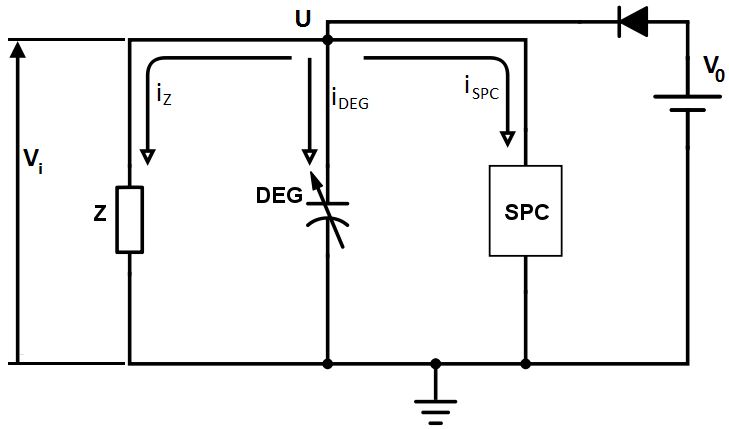
\includegraphics[height=4cm]{schemeit-project3.png}\\
\end{tabular}
\end{center}
\caption 
{ \label{fig:circuit}
Electronic circuit scheme of DEG-SPC system attached to a load.} 
\end{figure}

\subsection{Phase 1}

\paragraph{}  We consider the cycle starting from an initially charged state (provided by the source, $V_0$) and with the DEG relaxing from a stretched position that produces capacitance $C_{\text{DEG}_0}$.

\paragraph{} As explained previously, while the DEG relaxes, its capacitance is reduced and the voltage increases. No charge exchange happens between the SPC and the DEG, since the voltage is not large enough to trigger the HV form of the SPC. Meanwhile, some of the charge leaks  through the load (which represents either an energy harvesting impedance or simple losses/leakage in the system), resulting in
\begin{equation}
Q(t) = Q_0-\frac{V(t)}{Z} = V_0C_{\text{DEG}_0}-\frac{V(t)}{Z},
\end{equation}
where $Q(t)$ is the charge in the DEG and $Q_0$ is the charge level in the DEG provided by the voltage source $V_0$.  The voltage in Phase 1, $V_1$, will them vary with time as
\begin{equation}\label{eq:v1t}
V_{1}(t) = V_0\left(\frac{C_{\text{DEG}_0}}{C_\text{DEG}(t)+t/Z}\right).
\end{equation}


\paragraph{} As the voltage increases, it reaches the level held by the SPC in its high voltage form, $V_{\text{SPC}_\text{HV}}$. At this point we transition to the next phase, in which the DEG starts discharging into the SPC. The DEG state in which the transition occurs at a time $t_{12}$, which can be found as the first solution of  $V_1(t_{12}) = V_{\text{SPC}_\text{HV}}$. From Equation \ref{eq:v1t} this is equivalent to
\begin{equation}
V_{\text{SPC}_\text{HV}} = V_0\left(\frac{C_{\text{DEG}_0}}{C_\text{DEG}(t_{12})+t_{12}/Z}\right).
\end{equation}


\subsubsection{Phase 2}

\paragraph{} During Phase 2, the DEG voltage increases and not only supplies current to the load but also discharges into the SPC in its HV form. To describe the voltage behavior, we start by writing Kirchhoff's current law for the node U (see Figure \ref{fig:circuit}) in a general case:
\begin{equation}\label{eq:kirchoff}
 \frac{V(t)}{Z} + C_\text{SPC}\diff{V(t)}{t}+C_\text{DEG}(t)\diff{V(t)}{t}+V(t)\diff{C_\text{DEG}(t)}{t} = 0.
\end{equation}

\paragraph{} Given that $C_\text{SPC} =C_{\text{SPC}_\text{HV}}$ in this phase, and considering the initial conditions of this phase $C_\text{DEG}(t_{12}) = C_{\text{DEG}_{12}}$ and $V(t_{12}) = V_{\text{SPC}_\text{HV}}$, Equation \ref{eq:kirchoff} can be solved to give us the voltage in Phase 2, $V_2(t)$, as
\begin{equation}\label{eq:v2t}
V_2(t) = V_{\text{SPC}_\text{HV}}\left(\frac{C_{\text{SPC}_\text{HV}}+C_{\text{DEG}_{12}}}{C_{\text{SPC}_\text{HV}}+C_\text{DEG}(t)}\right)e^{\beta_2(t)},
\end{equation}
where
\begin{equation}
\diff{\beta_2}{t} = -\frac{1}{Z(C_{\text{SPC}_\text{HV}}+C_\text{DEG}(t))}.
\end{equation}

\paragraph{}The peak voltage can then be found when the DEG capacitance reaches its minimum value, by using $C_\text{DEG}(t_{23}) = C_{\text{DEG}_\text{min}}$, noting that $t_{23}$ marks the transition time to Phase 3.


\subsection{Phase 3}

\paragraph{} After reaching its maximum voltage, the DEG starts being stretched again and its capacitance increases, leading to a voltage drop. The current through the SPC ceases, since its voltage in the HC form is higher than that of the DEG. Thus, there is only current from the DEG to the attached load, as in Phase 1. Now, the voltage drops from the peak voltage, $V_\text{max}$ achieved when the DEG reaches its minimal capacitance, $C_{\text{DEG}_\text{min}}$. Using the same approach as before, we obtain
\begin{equation}\label{eq:v3t}
V_{3}(t) = V_\text{max}\left(\frac{C_{\text{DEG}_\text{min}}}{C_\text{DEG}(t)+t/Z}\right).
\end{equation}

\paragraph{} As the voltage drops, it will reach the potential of the SPC in its HC state, $V_{\text{SPC}_\text{HC}}$, at time $t=t_{34}$, and, at this point, we have a transition to the next phase. We can find the DEG state based on its capacitance when the DEG will start charging up using the energy stored in the SPC, $C_{\text{DEG}_{34}} = C_\text{DEG}(t_{34})$. Substituting into Equation \ref{eq:v3t}, we have
\begin{equation}
V_{\text{SPC}_\text{HC}} = V_\text{max}\left(\frac{C_{\text{DEG}_\text{min}}}{C_{\text{DEG}_{34}}+t_{34}/Z}\right).
\end{equation}

\subsection{Phase 4}

\paragraph{} During Phase 4, the DEG voltage reaches the SPC voltage in its HC form and starts charging up from it. As this phase uses the same circuit analyzed in Phase 2, we use again the generalized Equation \ref{eq:kirchoff} as a starting point. We apply the initial conditions for the phase transition at $t_{34}$, and obtain that
\begin{equation}\label{eq:v4t}
V_4(t) = V_{\text{SPC}_\text{HC}}\left(\frac{C_{\text{SPC}_\text{HC}}+C_{\text{DEG}_{34}}}{C_{\text{SPC}_\text{HC}}+C_\text{DEG}(t)}\right)e^{\beta_4(t)},
\end{equation}
with
\begin{equation}
\diff{\beta_4}{t} = -\frac{1}{Z(C_{\text{SPC}_\text{HC}}+C_\text{DEG}(t))}.
\end{equation}

\subsection{Following cycle}

\paragraph{} From Equation \ref{eq:v4t}, we can see clearly that a local minimum will be obtained using the maximum value of $C_\text{DEG}(t)$.	As the voltage curve reaches this local minimum, we return to phase 1 of the cycle, but this time using the DEG's maximum capacitance and the minimum voltage from the previous cycle as initial conditions.

\section{Modeling voltage boost}

\paragraph{} Given the model described above, we study a case focused on boosting the voltage, without concerns regarding energy output through external loads and neglecting the effects of non ideal elements. Thus, we obtain a simplified version of the model by  neglecting  the attached impedance, $Z$, considering it infinite and ignoring the current drained through it.

\subsection{Simplified model}\label{sec:noload}

\paragraph{} Through Equations \ref{eq:v1t}, \ref{eq:v2t}, \ref{eq:v3t} and \ref{eq:v4t} we have described the DEG-SPC system cycle considering current drained through a load with impedance $Z$. If we consider $Z\rightarrow\infty$ and that it is not the first cycle to run, we can define the voltage behavior as a new function, $V^\star(t)$, which is given in each of the phases described previously by:
\begin{align}
V_{1}^\star(t) &= V_\text{min}\left(\frac{C_{\text{DEG}_\text{max}}}{C_\text{DEG}(t)}\right), \label{V1star}\\
V_2^\star(t) &= V_{\text{SPC}_\text{HV}}\left(\frac{C_{\text{SPC}_\text{HV}}+C_{\text{DEG}_{12}}}{C_{\text{SPC}_\text{HV}}+C_\text{DEG}(t)}\right), \label{V2star}\\
V_{3}^\star(t) &= V_\text{max}\left(\frac{C_{\text{DEG}_\text{min}}}{C_\text{DEG}(t)}\right),\label{V3star}\\ 
V_4^\star(t) &= V_{\text{SPC}_\text{HC}}\left(\frac{C_{\text{SPC}_\text{HC}}+C_{\text{DEG}_{34}}}{C_{\text{SPC}_\text{HC}}+C_\text{DEG}(t)}\right), \label{V4star}
\end{align}
where $V_\text{min}$ corresponds to the local  minimum in the DEG voltage curve achieved at the end of Phase 4 and $V_\text{max}$ the local maximum voltage obtained at the end of Phase 2.

\paragraph{} Following the same approaching and neglecting the current through the impedance, we can also describe the capacitances in the DEG at the transition between phases:
\begin{align}
C_{\text{DEG}_{12}} &= \frac{V_\text{min}C_{\text{DEG}_\text{max}}}{V_{\text{SPC}_\text{HV}}},\\
C_{\text{DEG}_{34}} &= \frac{V_\text{max}C_{\text{DEG}_\text{min}}}{V_{\text{SPC}_\text{HC}}},
\end{align}
where, in this scenario,
\begin{align}
{V_{\text{SPC}_\text{HV}}} &=  \frac{n+1}{n}V_\text{min}\\
{V_{\text{SPC}_\text{HC}}} &=  \frac{n}{n+1}V_\text{max}.
\end{align}

\subsection{Voltage boost model}

\paragraph{} We say that there has been a voltage boost if the peak voltage in a cycle is higher than the peak in the previous one. We evaluate the boost through the parameter $B$, defined as the ratio between a maximum voltage in a cycle and that of the previous one. The set of equations described in Section \ref{sec:noload} allows us to determine the relation between a local maximum in the voltage curve for a cycle, $V_{\text{max}_{j}}$ and the process can be extended to the next local maximum, $V_{\text{max}_{j+1}}$, located in the following cycle. The equation can be broken down using the basic parameters $C$ and $n$, which reflect the SPC design, and the DEG capacitance swing between minimum capacitance, $C_{\text{DEG}_\text{min}}$, and maximum capacitance, $C_{\text{DEG}_\text{max}}$, yielding
\begin{equation}\label{eq:boost}
B = \frac{V_{\text{max}_{j+1}}}{V_{\text{max}_{j}}}=\frac{C^{2}+(C_{\text{DEG}_{\min}}+C_{\text{DEG}_{\max}})C+C_{\text{DEG}_{\min}}C_{\text{DEG}_{\max}}}{C^{2}+\left(\dfrac{n^{2}C_{\text{DEG}_{\max}}+(n+1)^{2}C_{\text{DEG}_{\min}}}{n(n+1)}\right)C+C_{\text{DEG}_{\min}}C_{\text{DEG}_{\max}}}.
\end{equation}

\paragraph{} Equation \ref{eq:boost} provides insights about several aspects of system design and behavior. First, it allows us to verify the minimum requirements for boost to exist, when $B >1$. It can also be seen that the ratio between maximum voltage in a cycle and that of the previous one stays constant if both the SPC  characteristics, and the DEG capacitance swing, are maintained. Another possibility is verifying the design parameters that lead to a maximum boost, which can be achieved easily by differentiation. We can search for the value of $C$ that maximizes the boost and also determine how increasing the number of stages, $n$, affects the SPC.


\subsubsection{Condition for boost to exist}
\paragraph{} To obtain boost, we must have $B>1$, which leads us straightforwardly to the condition
\begin{equation}\label{eq:ncond}
n > \frac{1}{C_{\text{DEG}_\text{max}}/C_{\text{DEG}_\text{min}}-1}.
\end{equation}

\subsubsection{Maximum boost}

\paragraph{} In order to choose the value of $C$ which will provide the maximum boost, $B$, we seek solutions of $\odiff{B}{C}=0$, which gives
\begin{equation}\label{eq:bestC}
C= \sqrt{C_{\text{DEG}_{\text{min}}}C_{\text{DEG}_{\text{max}}}}.
\end{equation}

\paragraph{} We can see in Figure \ref{fig:boost} the importance of selecting the right value of $C$, as the voltage could even decrease at each cycle if inappropriately chosen. If the capacitance of the SPC is too high, the capacitance swing from the DEG would be negligible when compared to the SPC's  capacitance; the Phase 2 voltage rise would stop as all the charges would flow from the DEG to the SPC instead of increasing the voltage. On the other hand, if the SPC capacitance is too low, it would not be able to accommodate enough charge to keep the boosting process going. In this case, we would have a voltage swing due exclusively to a DEG capacitance change when it holds constant charge, having only Phases 1 and 3 of the cycle (Equations \ref{V2star} and \ref{V4star} would converge to Equations \ref{V1star} and \ref{V3star}). It is also possible to verify how relevant the capacitance change, evaluate hered as $C_{\text{DEG}_\text{max}}/C_{\text{DEG}_\text{min}}$ is, as its effect on the voltage boost is clearly visible in Figure \ref{fig:boost}. The higher the capacitance change, the higher the maximum voltage boost possible.

\begin{figure}[ht]
\begin{center}
\begin{tabular}{c}
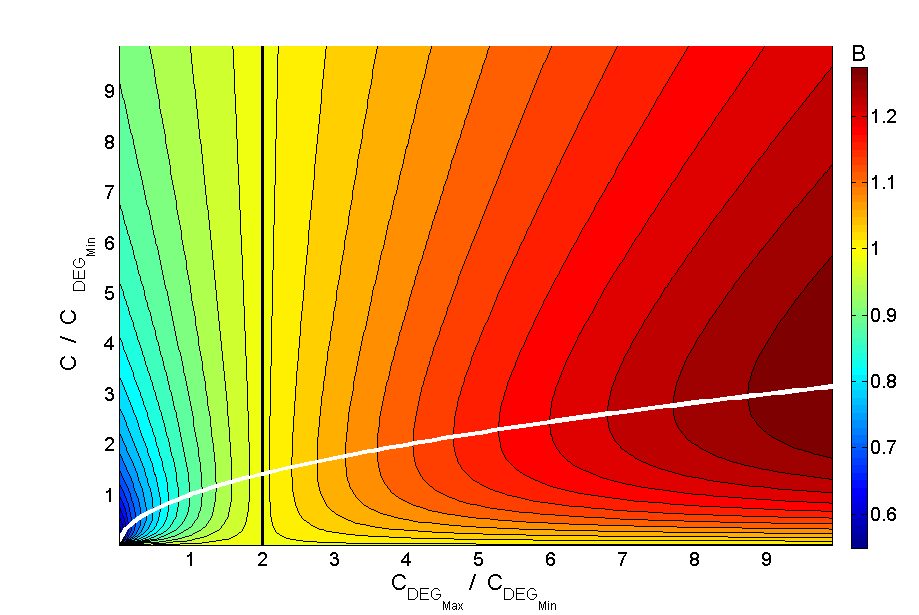
\includegraphics[height=9cm]{boostmap2.png}\\
\end{tabular}
\end{center}
\caption 
{ \label{fig:boost}
Voltage boost, $B$, shown as a function of DEG capacitance change, $C_{\text{DEG}_{\max}}/C_{\text{DEG}_{\min}}$, for different SPC base capacitance, $C$, for a one stage SPC ($n=1$). The white line indicates the peak boost as suggested by Equation \ref{eq:bestC}. The thick black line corresponds to $B=1$ and separates the region with boost (right) from that where the condition in Equation \ref{eq:ncond} is not fulfilled  and $B<1$ (left)}
\end{figure}



\subsubsection{Effect of the number of stages}

\paragraph{} The number of stages will influence the denominator of Equation \ref{eq:boost}, specifically the coefficient $A$ of the linear term in $C$,
\begin{equation}
A = \frac{n^{2}C_{\text{DEG}_{\max}}+(n+1)^{2}C_{\text{DEG}_{\min}}}{n(n+1)}.
\end{equation}
It is trivial to observe that if $n\rightarrow\infty$, $A\rightarrow C_{\text{DEG}_{\max}}+C_{\text{DEG}_{\min}}$, hence,  the denominator  of Equation \ref{eq:boost} becomes the same as the numerator and there is no boost.
We can find the number of stages that maximises the boost by solving $\odiff{B}{n}=0$ for $n$, and comparing the values of $B$ for the two integers either side of the turning point.
We can also verify that the maximum boost is obtained for $n=1$ if $\ofrac{C_{\text{DEG}_\text{max}}}{C_{\text{DEG}_\text{min}}}>3$. On the other hand, Figure \ref{fig:nvariation} illustrates how increasing the number of stages allows the boost to exist in a broader range of situations, when the capacitance swing is reduced, though it also shows a reduction in the voltage boost. This can be explained by the decrease in the difference of the SPC capacitance when toggled between its HV and HC forms, decreasing its effectiveness. Looking back at Equations \ref{eq:cspchv} and \ref{eq:cspchc}, the more stages are used, the closer the SPC effect becomes of that of a simple capacitor with capacitance $C$.

\begin{figure}[ht]
\begin{center}
\begin{tabular}{c}
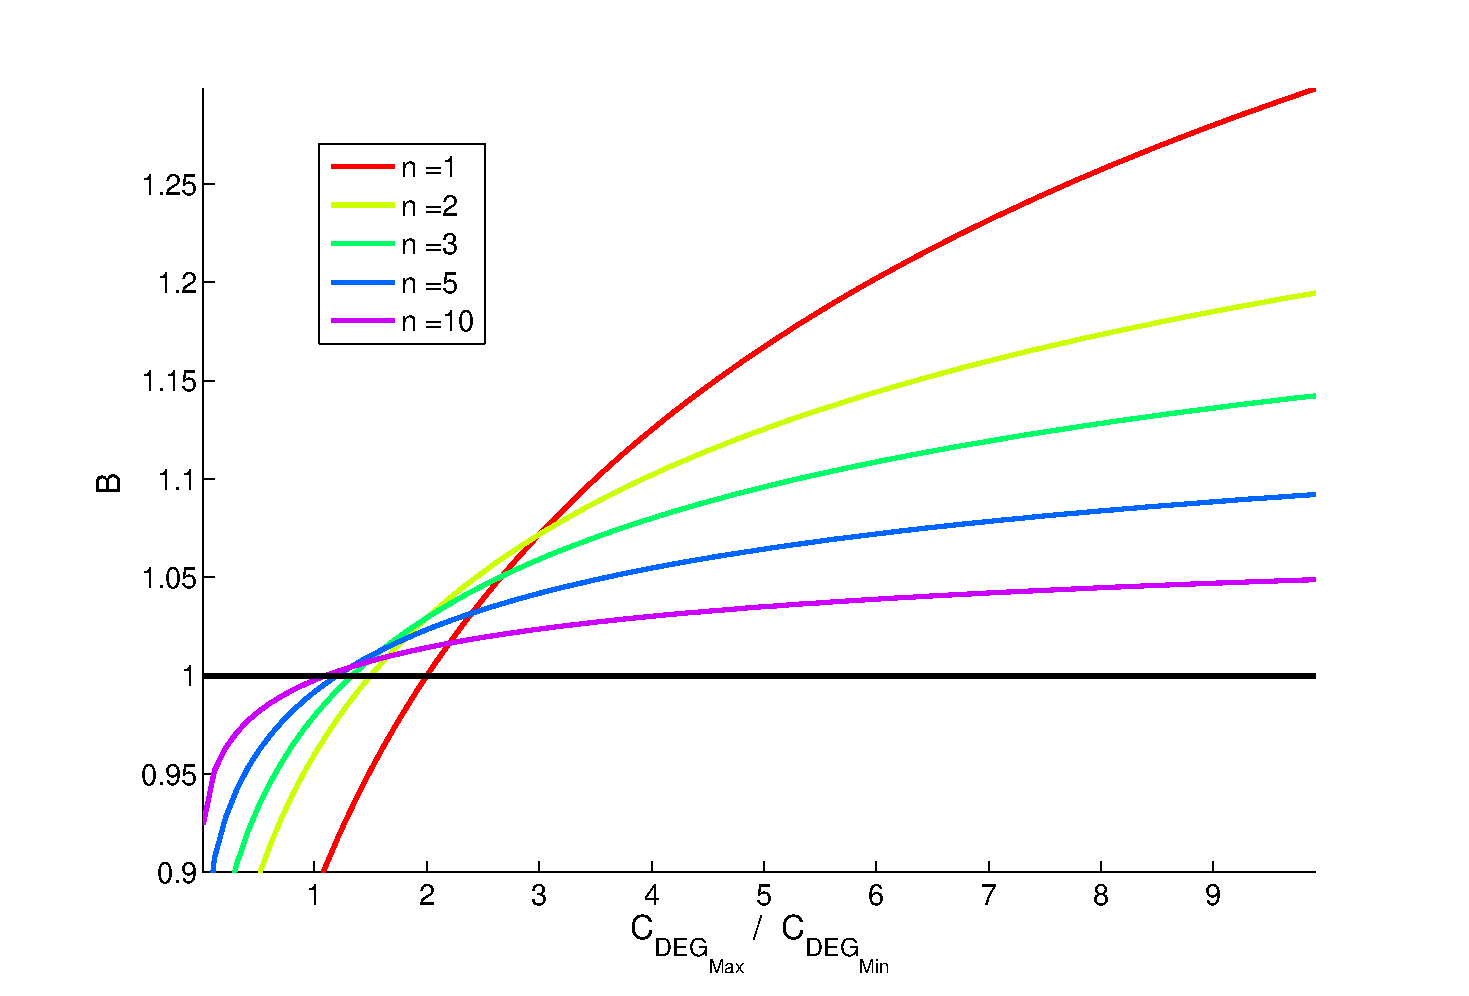
\includegraphics[height=9cm]{stages2.eps}\\
\end{tabular}
\end{center}
\caption 
{ \label{fig:nvariation}
Voltage boost, $B$, versus the DEG's capacitance swing, $\ofrac{C_{\text{DEG}_\text{max}}}{C_{\text{DEG}_\text{min}}}$, for different numbers of stages, $n$. The black line corresponds to $B=1$, and separates the region with boost (above) from that without (below).} 
\end{figure}

\section{Model validation}

\paragraph{} In order to validate the model, we compared its results with those obtained through the already validated model by McKay in LT Spice \cite{Thesis}. The model was built with a one-stage SPC ($n=1$) using capacitors of \SI{1}{\nano\farad}. The DEG's capacitance oscillated in a cycle between \SI{2}{\nano\farad} and \SI{8}{\nano\farad}. The circuit was initially primed at \SI{5}{\volt}. Only ideal elements were used and no load was considered (both for the present model and in the circuit). Figure \ref{fig:valid} shows that the model agrees very well with the LT Spice simulation with errors of less than 0.5\%.

\begin{figure}[ht]
\begin{center}
\begin{tabular}{c}
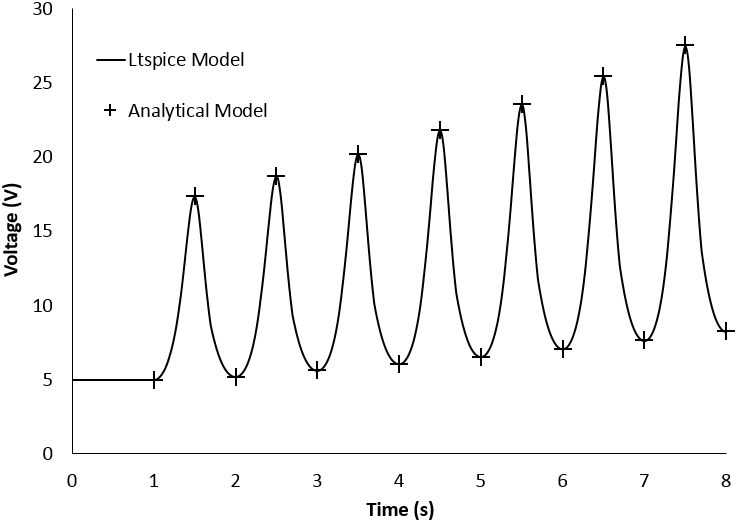
\includegraphics[height=7cm]{Modelcomparison3.PNG}\\
\end{tabular}
\end{center}
\caption 
{ \label{fig:valid}
Comparison of the voltage curve for LT Spice model (black line) and the maximum/minimum values obtained through the analytical method (crosses).} 
\end{figure}

\paragraph{} Another important point that validates the current analysis is the correspondence with the rules proposed in McKay \textit{et al.}\cite{SPCdesign}. There, it was suggested that $C$ and $n$ should be chosen such that
\begin{equation}
C_{SPC{HC}} = C_{\text{DEG}_\text{max}},
\end{equation}
and
\begin{equation}
\frac{(n+1)}{n} = \sqrt[]{\frac{C_{\text{DEG}_\text{max}}}{C_{\text{DEG}_\text{min}}}}.
\end{equation}
Uniting both of these conditions, we get to the same choice of $C$  expressed in Equation \ref{eq:bestC}. In addition, $n$ is chosen in a way that will necessarily obey the condition expressed in Equation \ref{eq:ncond}. In contrast, using Equation  \ref{eq:bestC} and observing the condition in Equation \ref{eq:ncond},  we are able to choose the parameters $C$ and $n$ independently.


\section{Conclusion}
\paragraph{} We have developed an analytical model that describes the physics behind each phase of the cycle of a DEG-SPC system with a load attached to it. Based on this model, we obtained a simplified version, from which we derived a simple closed-form analytic expression that describes the boost  per cycle of the DEG-SPC system. From this, we derived the condition for the boost to exist, the ideal parameters for the SPC, and also demonstrated how their variation affects the final voltage boost. In addition, we validated the simplified model by comparing it with another previously validated model\cite{Thesis} showing very good agreement. We have also provided a theoretical basis for the understanding of the SPC design rules previously proposed\cite{SPCdesign}. 


%=========================================================